%%%%%%%%%%%%%%%%%%%%%%%%%%%%%%%%%%%%%%%%%%%%%%%%%%%%%%%%%%%%%%%%%%%%%%%%%%%%%%%%
% Template for USENIX papers.
%
% History:
%
% - TEMPLATE for Usenix papers, specifically to meet requirements of
%   USENIX '05. originally a template for producing IEEE-format
%   articles using LaTeX. written by Matthew Ward, CS Department,
%   Worcester Polytechnic Institute. adapted by David Beazley for his
%   excellent SWIG paper in Proceedings, Tcl 96. turned into a
%   smartass generic template by De Clarke, with thanks to both the
%   above pioneers. Use at your own risk. Complaints to /dev/null.
%   Make it two column with no page numbering, default is 10 point.
%
% - Munged by Fred Douglis <douglis@research.att.com> 10/97 to
%   separate the .sty file from the LaTeX source template, so that
%   people can more easily include the .sty file into an existing
%   document. Also changed to more closely follow the style guidelines
%   as represented by the Word sample file.
%
% - Note that since 2010, USENIX does not require endnotes. If you
%   want foot of page notes, don't include the endnotes package in the
%   usepackage command, below.
% - This version uses the latex2e styles, not the very ancient 2.09
%   stuff.
%
% - Updated July 2018: Text block size changed from 6.5" to 7"
%
% - Updated Dec 2018 for ATC'19:
%
%   * Revised text to pass HotCRP's auto-formatting check, with
%     hotcrp.settings.submission_form.body_font_size=10pt, and
%     hotcrp.settings.submission_form.line_height=12pt
%
%   * Switched from \endnote-s to \footnote-s to match Usenix's policy.
%
%   * \section* => \begin{abstract} ... \end{abstract}
%
%   * Make template self-contained in terms of bibtex entires, to allow
%     this file to be compiled. (And changing refs style to 'plain'.)
%
%   * Make template self-contained in terms of figures, to
%     allow this file to be compiled. 
%
%   * Added packages for hyperref, embedding fonts, and improving
%     appearance.
%   
%   * Removed outdated text.
%
%%%%%%%%%%%%%%%%%%%%%%%%%%%%%%%%%%%%%%%%%%%%%%%%%%%%%%%%%%%%%%%%%%%%%%%%%%%%%%%%

\documentclass[letterpaper,twocolumn,10pt]{article}
\usepackage{usenix2019_v3}

% to be able to draw some self-contained figs
\usepackage{hyperref}
\usepackage{tikz}
\usepackage{amsmath}
\usepackage{tabularx}

%-------------------------------------------------------------------------------
\begin{document}
%-------------------------------------------------------------------------------

%don't want date printed
\date{}

\title{\Large Adversarial Obfuscation for Domain Fronting}

\author{
{\rm Steven R. Sheffey}\\
Middle Tennessee State University
\and
{\rm Ferrol Aderholdt}\\
Middle Tennessee State University
} % end author

\maketitle

%-------------------------------------------------------------------------------
\begin{abstract}
%-------------------------------------------------------------------------------
% Your abstract text goes here. Just a few facts. Whet our appetites.
% Not more than 200 words, if possible, and preferably closer to 150.
As the becomes more important as a source of information, internet censorship has become more pervasive. Tor aims to circumvent censorship, but adversaries are capable of blocking Tor traffic. Pluggable transports are used to obfuscate tor traffic to circumvent this. Meek uses domain fronting to emulate benign and trusted HTTPS traffic, with the hope that adversaries will avoid blocking it in order to avoid the collateral damage of blocking a reputable website. However, attacks using machine learning to differentiate domain-fronted traffic from regular HTTPS traffic pose a threat to the effectiveness of domain fronting. We propose the use of adversarial machine learning to model and reduce this threat.
\end{abstract}


%-------------------------------------------------------------------------------
\section{Introduction}
%-------------------------------------------------------------------------------
foo
\nocite{*}


%-------------------------------------------------------------------------------
\section{Background}
%-------------------------------------------------------------------------------

\subsection{Censorship}
\begin{itemize}
    \item Internet censorship has become pervasive (china, iran, saudi arabia, russia, etc)
    \item The Tor network is used to circumvent internet censorship
    \item Censors have blocked Tor
\end{itemize}
\subsection{Obfuscation}
Obfuscators are used to circumvent protocol censorship or increase privacy. Tor uses Pluggable Transports
\subsubsection{Forms of Obfuscation}

\begin{itemize}
    \item Randomization (obfsproxy, scramblesuit)
    \item Mimicry (Skypemorph, Marionette, FTE)
    \item Tunneling (Meek)
    \item Traffic shaping, chaff
    \item TODO: snowflake, other newer obfuscators
\end{itemize}
TODO: go into detail about meek

\subsubsection{Attacks against Obfuscation}
\begin{itemize}
    \item Syntactic/Semantic (badly obfuscated traffic doesn't make sense semantically in its transformed protocol)
    \item Entropy
    \item Traffic statistical analysis
    \item TODO: others
\end{itemize}

TODO: go into detail about statistical analysis/machine learning

Wang et al \cite{Wang:2015:STN:2810103.2813715} were able to identify Meek traffic with a FPR (false positive rate) of 0.0002 on meek-amazon and 0.00006 on meek-google. This indicates that traffic analysis attacks using machine learning pose a major threat to traffic obfuscation and anti-censorship efforts.

%-------------------------------------------------------------------------------
\section{Related Work}
TODO: talk about wang et al

TODO: find more papers identifying tor with machine learning

TODO: talk about the other adversarial transformation paper

\section{Data Collection}
We implement a framework that allows for reproducible, parallel generation of packet captures for HTTPS traffic with and without tor and pluggable transports.
\subsection{Framework}
\begin{figure}
    \begin{center}
        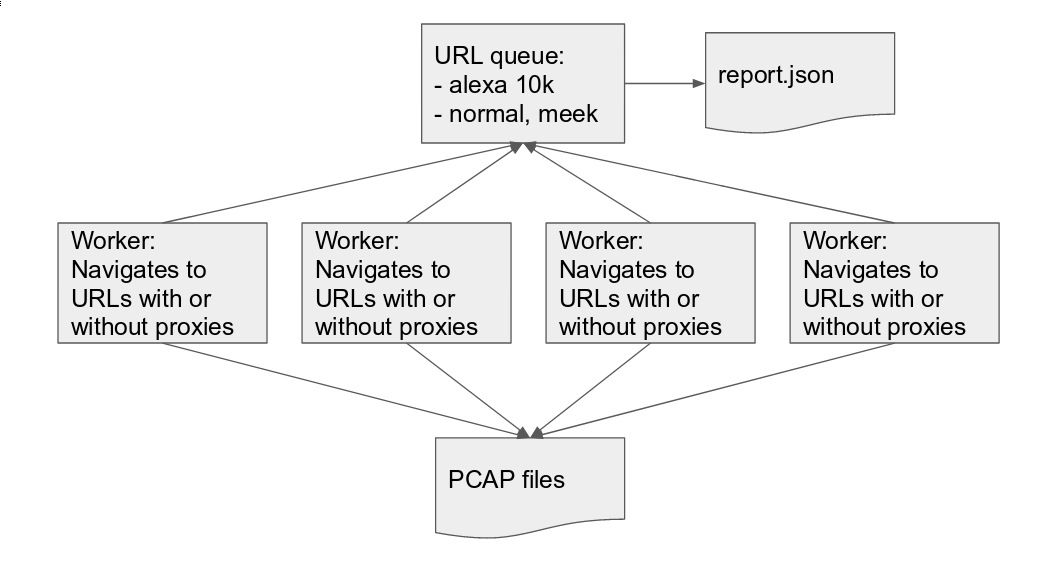
\includegraphics[width=0.5\textwidth]{figures/data-collection-architecture}
    \end{center}
    \caption{\label{fig:data-collection-architecture} Architecture of data collection containers} 
\end{figure}
\subsection{Datasets}
Each of our datasets contains packet captures for navigating to the top 10000 websites of the Alexa top 1M %\cite{TODO: alexa}. 
both without any proxies, and through Tor over Meek. The meek server used is through meek-azure.
We collect datasets from a home wired network ($H_{normal}$, $H_{meek}$), a university wired network ($U_{normal}$, $U_{meek}$), and an AWS \texttt{m5.2xlarge} instance ($A_{normal}$, $A_{meek}$).
\subsection{Feature Extraction}
foo
\section{Adversarial Model}
\subsection{Architecture}
We use StarGAN \cite{Choi_2018_CVPR} as a basis for obfuscation. StarGAN allows for adversarial transformation through application of a variety of features, though for this model, we only use a binary set of features (Meek or normal). Additionally, StarGAN performs well on datasets from multiple domains, which has potential applications in transforming obfuscated traffic of multiple types or locations.
\begin{figure*}
    \begin{center}
        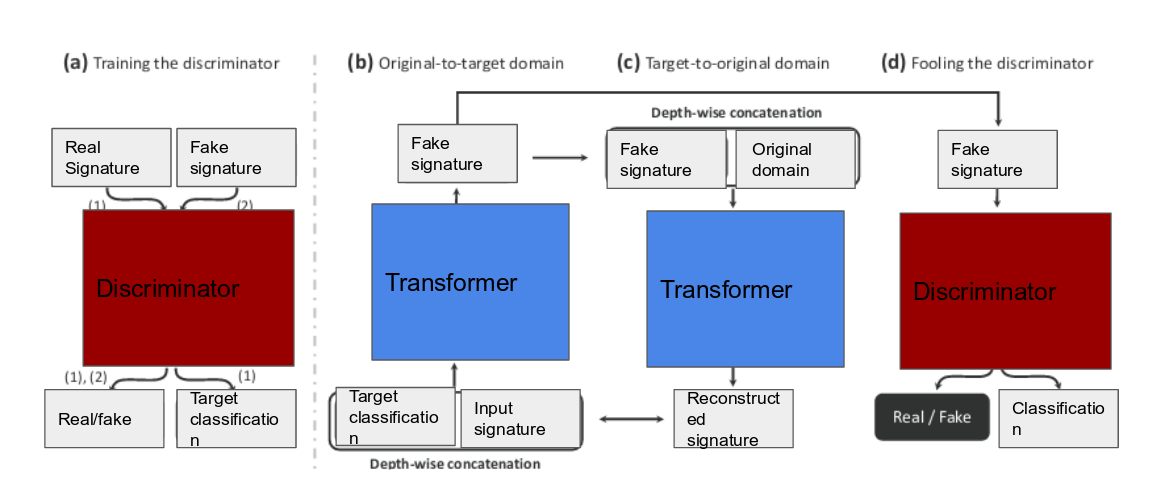
\includegraphics[width=\textwidth]{figures/stargan-architecture}
    \end{center}
    \caption{\label{fig:data-collection-architecture} Architecture of our adapted version of StarGAN} 
\end{figure*}
\subsection{Training and Evaluation}
foo
%-------------------------------------------------------------------------------
\section{Results}
%-------------------------------------------------------------------------------
\begin{figure}
    \begin{center}
        \begin{tabularx}{0.5\textwidth}{ |X|X|X|X| }
          \hline
            & Basline & Transformed & Transformed \& flipped class \\
          \hline 
          Classifier  & 0.99  & 0.3  & 0.99  \\
          \hline 
          Discriminator & 0.99  & 0.3  & 0.99  \\
          \hline
          Random Forest & 0.99  & 0.3  & 0.99  \\
          \hline
        \end{tabularx}
    \end{center}
    \caption{\label{fig:results-pr-auc} Effect of transformer on PR-AUC} 
\end{figure}
\begin{figure}
    \begin{center}
        \begin{tabularx}{0.5\textwidth}{ |X|X|X|X| }
          \hline
            & Basline & Transformed & Transformed \& flipped class \\
          \hline 
          Classifier  & 0.99  & 0.3  & 0.99  \\
          \hline 
          Discriminator & 0.99  & 0.3  & 0.99  \\
          \hline
          Random Forest & 0.99  & 0.3  & 0.99  \\
          \hline
        \end{tabularx}
    \end{center}
    \caption{\label{fig:results-fpr} Effect of transformer on FPR} 
\end{figure}
foo
%-------------------------------------------------------------------------------
\section{Conclusions}
%-------------------------------------------------------------------------------
Our results indicate that 
%-------------------------------------------------------------------------------
\section{Availability}
%-------------------------------------------------------------------------------

The traffic generation framework, feature extractor, and machine learning code for this work is open source, and can be accessed at \href{https://github.com/starfys/packet_captor_sakura}{\texttt{https://github.com/starfys/packet\_captor\_sakura}}
%-------------------------------------------------------------------------------
\bibliographystyle{plain}
\bibliography{paper}

%%%%%%%%%%%%%%%%%%%%%%%%%%%%%%%%%%%%%%%%%%%%%%%%%%%%%%%%%%%%%%%%%%%%%%%%%%%%%%%%
\end{document}
%%%%%%%%%%%%%%%%%%%%%%%%%%%%%%%%%%%%%%%%%%%%%%%%%%%%%%%%%%%%%%%%%%%%%%%%%%%%%%%%

%%  LocalWords:  endnotes includegraphics fread ptr nobj noindent
%%  LocalWords:  pdflatex acks
